\documentclass[calcdimensions,landscape,letterpaper]{powersem}
\usepackage{color}
\usepackage[pdftex]{thumbpdf} % For thumbnails
\usepackage[pdftex]{hyperref} % For links.
\usepackage[display,coloremph,whitebackground]{texpower} % colormath
\usepackage{fixseminar}
\usepackage{tpslifonts}
\usepackage[pdftex,final]{graphicx} % For including graphics.
\usepackage[utf8]{inputenc}
\usepackage{minted}
\usepackage{amsmath}
\usepackage{amssymb}
\usepackage{eurosym}
\usepackage{booktabs} % rules in tables
\usepackage{multirow} % multi-row cells
\usepackage{rotating} % text rotation

\title{A Short Introduction to OpenGL}
\author{Jan Wedekind}
\date{Thursday, May 30th 2024}

\DeclareGraphicsExtensions{.jpg,.pdf,.png}
\pdfcompresslevel=9

\hypersetup{
   pdftitle          = {\thetitle},
   pdfsubject        = {Short OpenGL Presentation 30th May 2024},
   pdfauthor         = {Jan Wedekind},
   pdfkeywords       = {opengl, graphics, software},
   pdfcreator        = {okular},
   pdfproducer       = {LaTeX with TexPower and Minted},
   bookmarksopen     = false,
   bookmarksnumbered = true,
   colorlinks        = true,
   pdfstartpage      = {1},
   pdfpagemode       = {FullScreen}
}

\DeclarePanel{top}{
  \begin{picture}(0,0)
    \put(-3, -293){\resizebox*{\pdfpagewidth}{\pdfpageheight}{
\includegraphics{slide.png}}}
    \put(-10,-20){\parbox[c]{.9\textwidth}{\center\large\bf\thecurrentheading}}
  \end{picture}
}

\DeclarePanel{bottom}{
  \begin{picture}(0,0)
    \put(0,15){\parbox[c]{.98\pdfpagewidth}{\tiny\thedate\hfill\theslide/37}}
  \end{picture}
}

\slidesmag{4}
\backgroundstyle{none}
\slideframe{none}
\pagestyle{empty}

\mklength{\slideleftmargin}{-2cm}
\mklength{\sliderightmargin}{-2cm}
\mklength{\slidetopmargin}{2.0cm}
\mklength{\slidebottommargin}{1.5cm}

\renewcommand{\currentpagevalue}{\value{slide}}
\newcommand{\thecurrentheading}{}
\newcommand{\heading}[1]{\renewcommand{\thecurrentheading}{#1}}
\newcommand{\subheading}[1]{\concept{#1}}

\begin{document}

\begin{slide}
  \pdfbookmark[1]{\thetitle}{title}
  \heading{\ }
  \begin{center}
    \maketitle
  \end{center}
\end{slide}

\begin{slide}
  \pdfbookmark[1]{Motivation}{motivation}
  \heading{Motivation}
  \begin{center}
    \resizebox*{.5\textwidth}{!}{
\includegraphics{logo}}\bigskip\\
    \begin{minipage}[c]{.95\textwidth}
      \begin{itemize}
          \item OpenGL is cross-platform
          \item OpenGL is less verbose than Vulkan, but OpenGL knowledge transferable to Vulkan
          \item OpenGL has bindings for many languages
      \end{itemize}
    \end{minipage}
  \end{center}
\end{slide}

\begin{slide}
  \pdfbookmark[1]{Showcase}{showcase}
  \heading{Showcase}
  \begin{center}
    \begin{minipage}[c]{.47\textwidth}
      \begin{center}
        \resizebox*{\textwidth}{!}{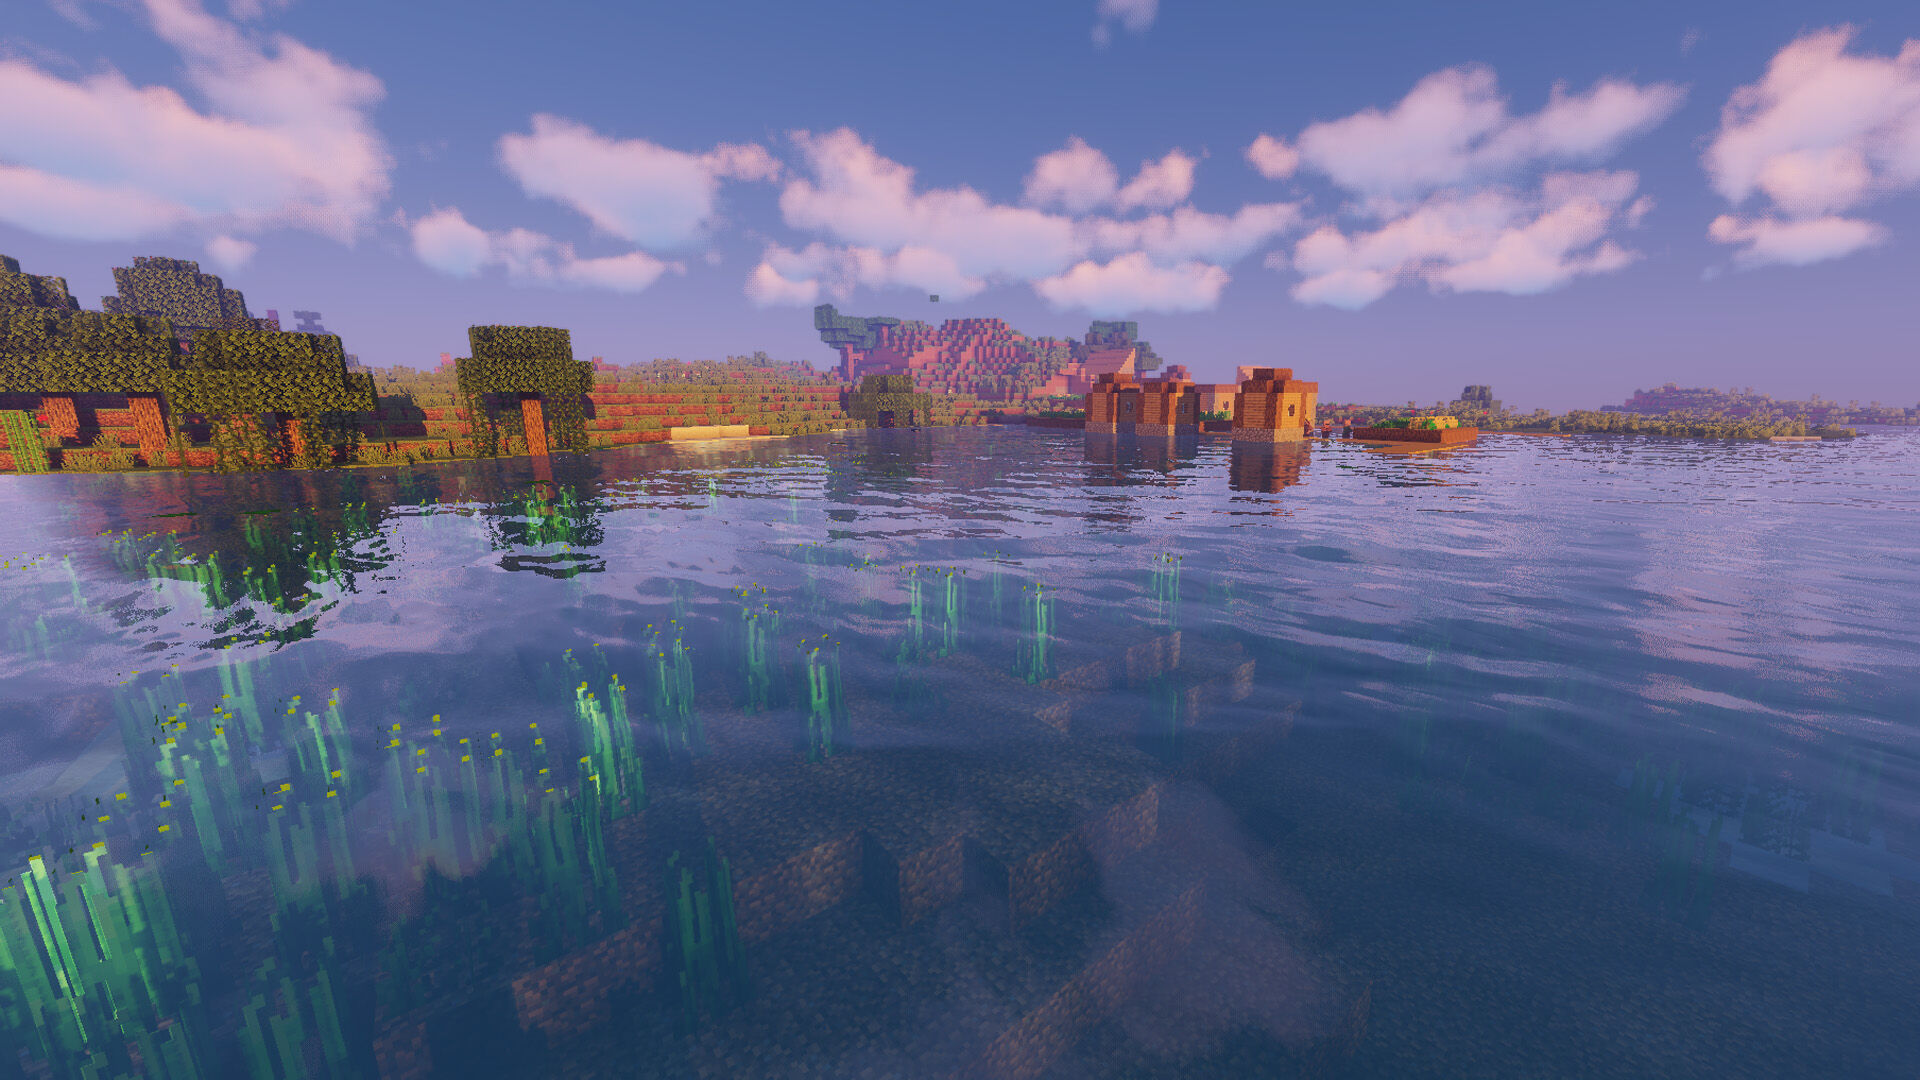
\includegraphics{minecraft}}\\
        Minecraft Java Edition
      \end{center}
    \end{minipage}
    \begin{minipage}[c]{.47\textwidth}
      \begin{center}
        \resizebox*{\textwidth}{!}{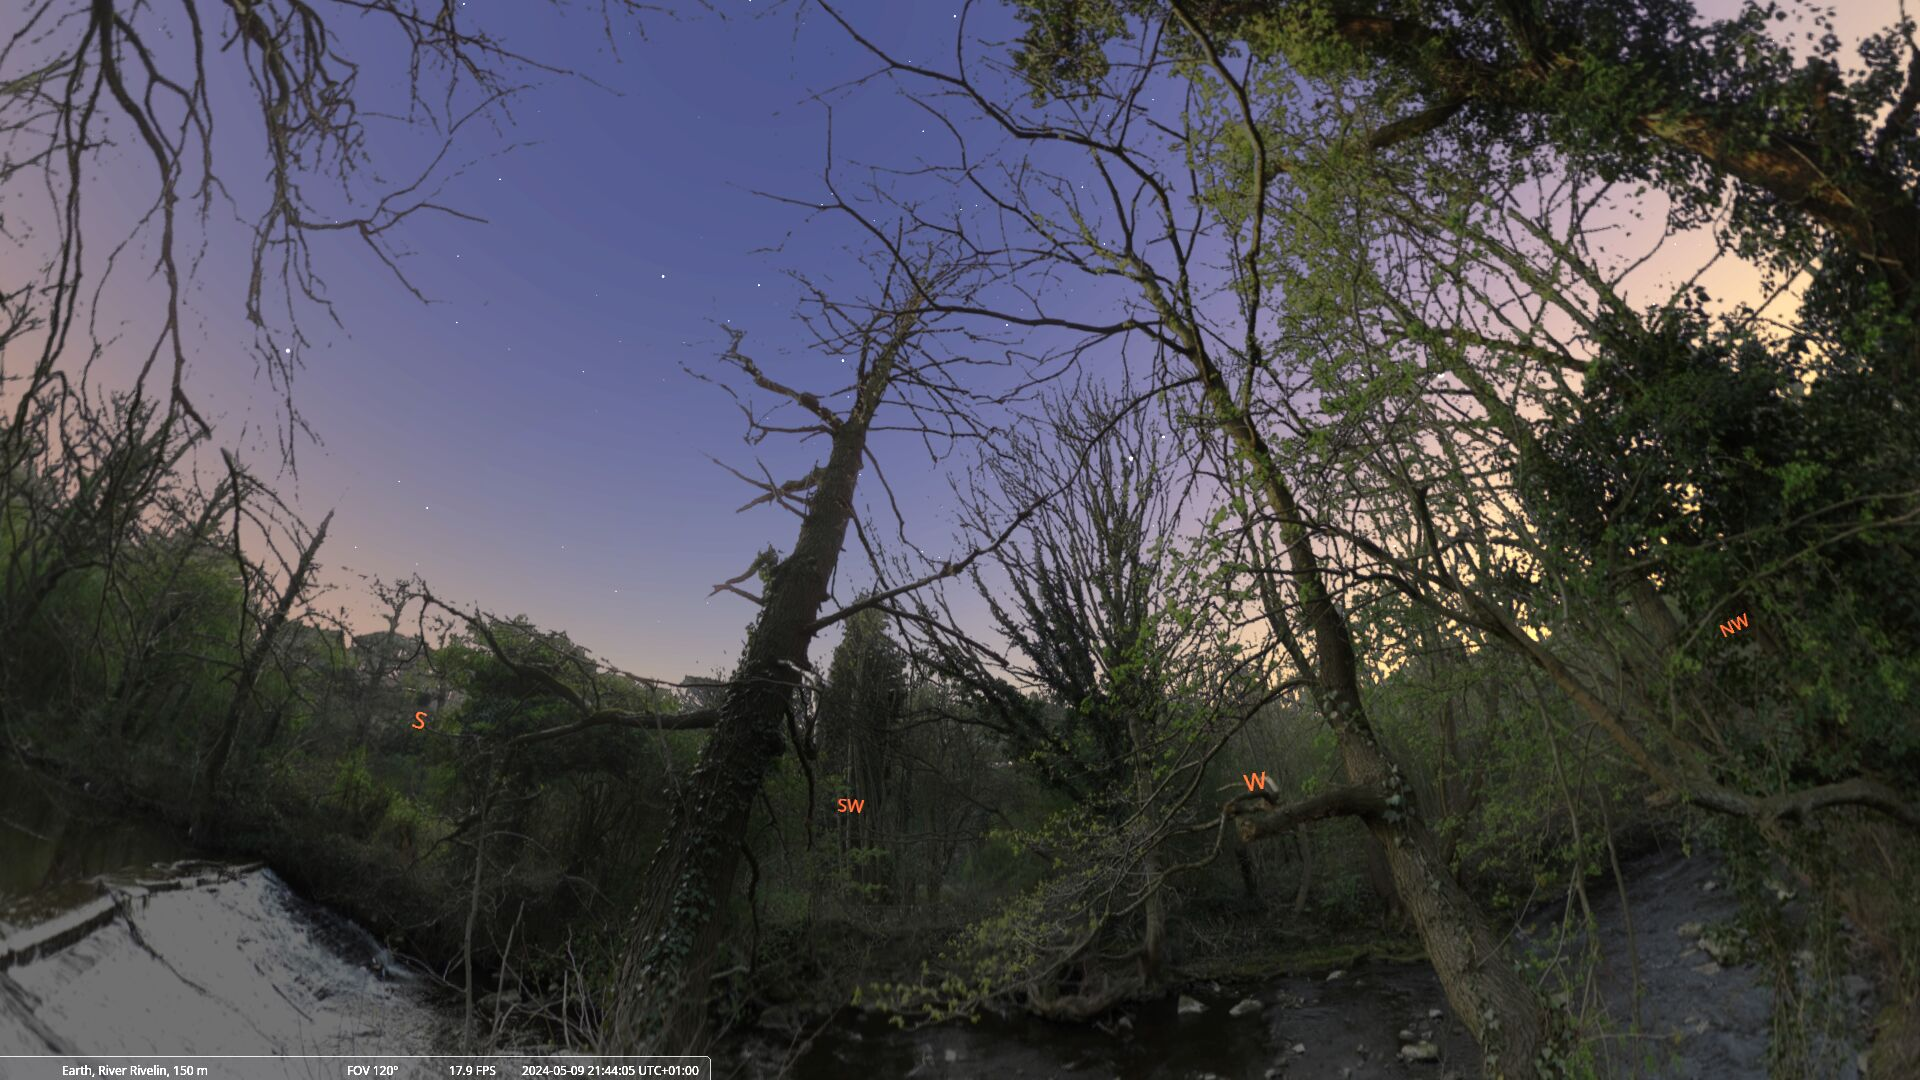
\includegraphics{stellarium}}\\
        Stellarium
      \end{center}
    \end{minipage}\bigskip\\
    \begin{minipage}[c]{.47\textwidth}
      \begin{center}
        \resizebox*{\textwidth}{!}{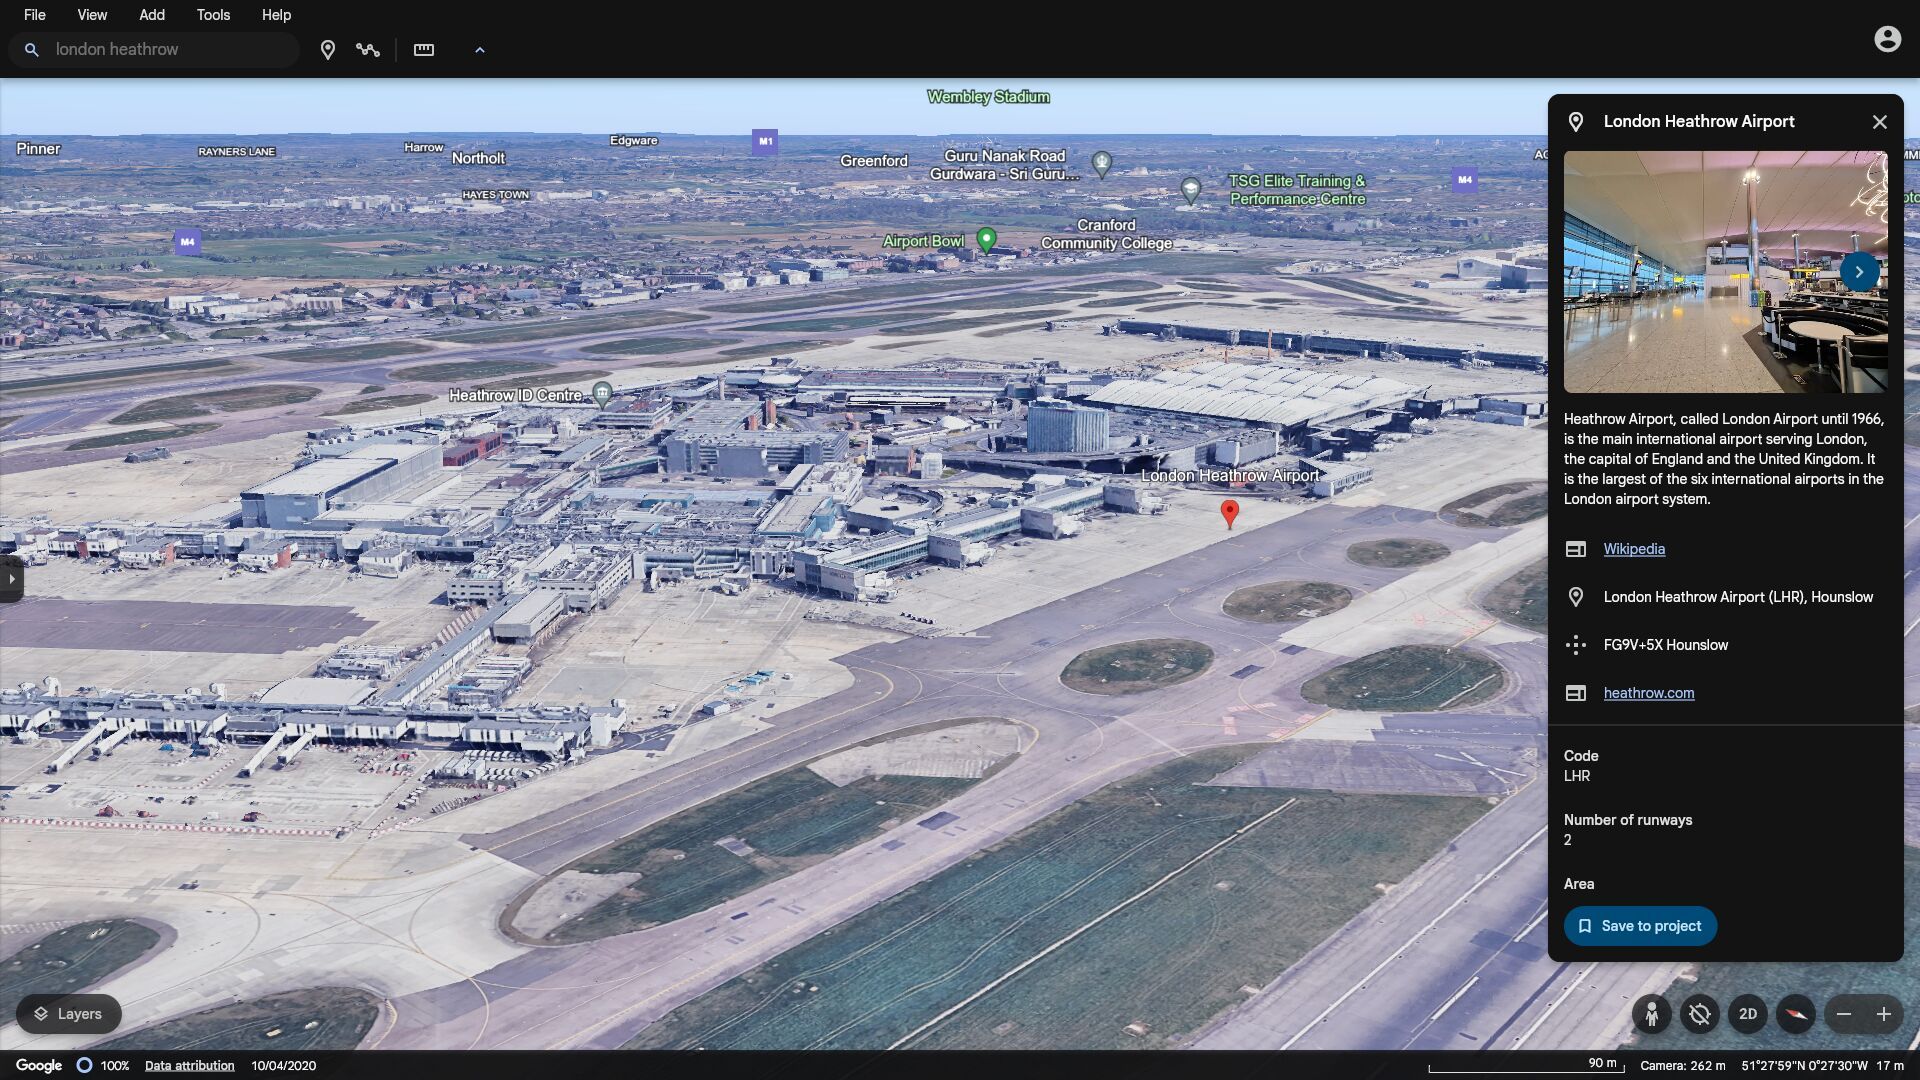
\includegraphics{google-earth}}\\
        WebGL (e.g. Google Earth)
      \end{center}
    \end{minipage}
    \begin{minipage}[c]{.47\textwidth}
      \begin{center}
        \resizebox*{\textwidth}{!}{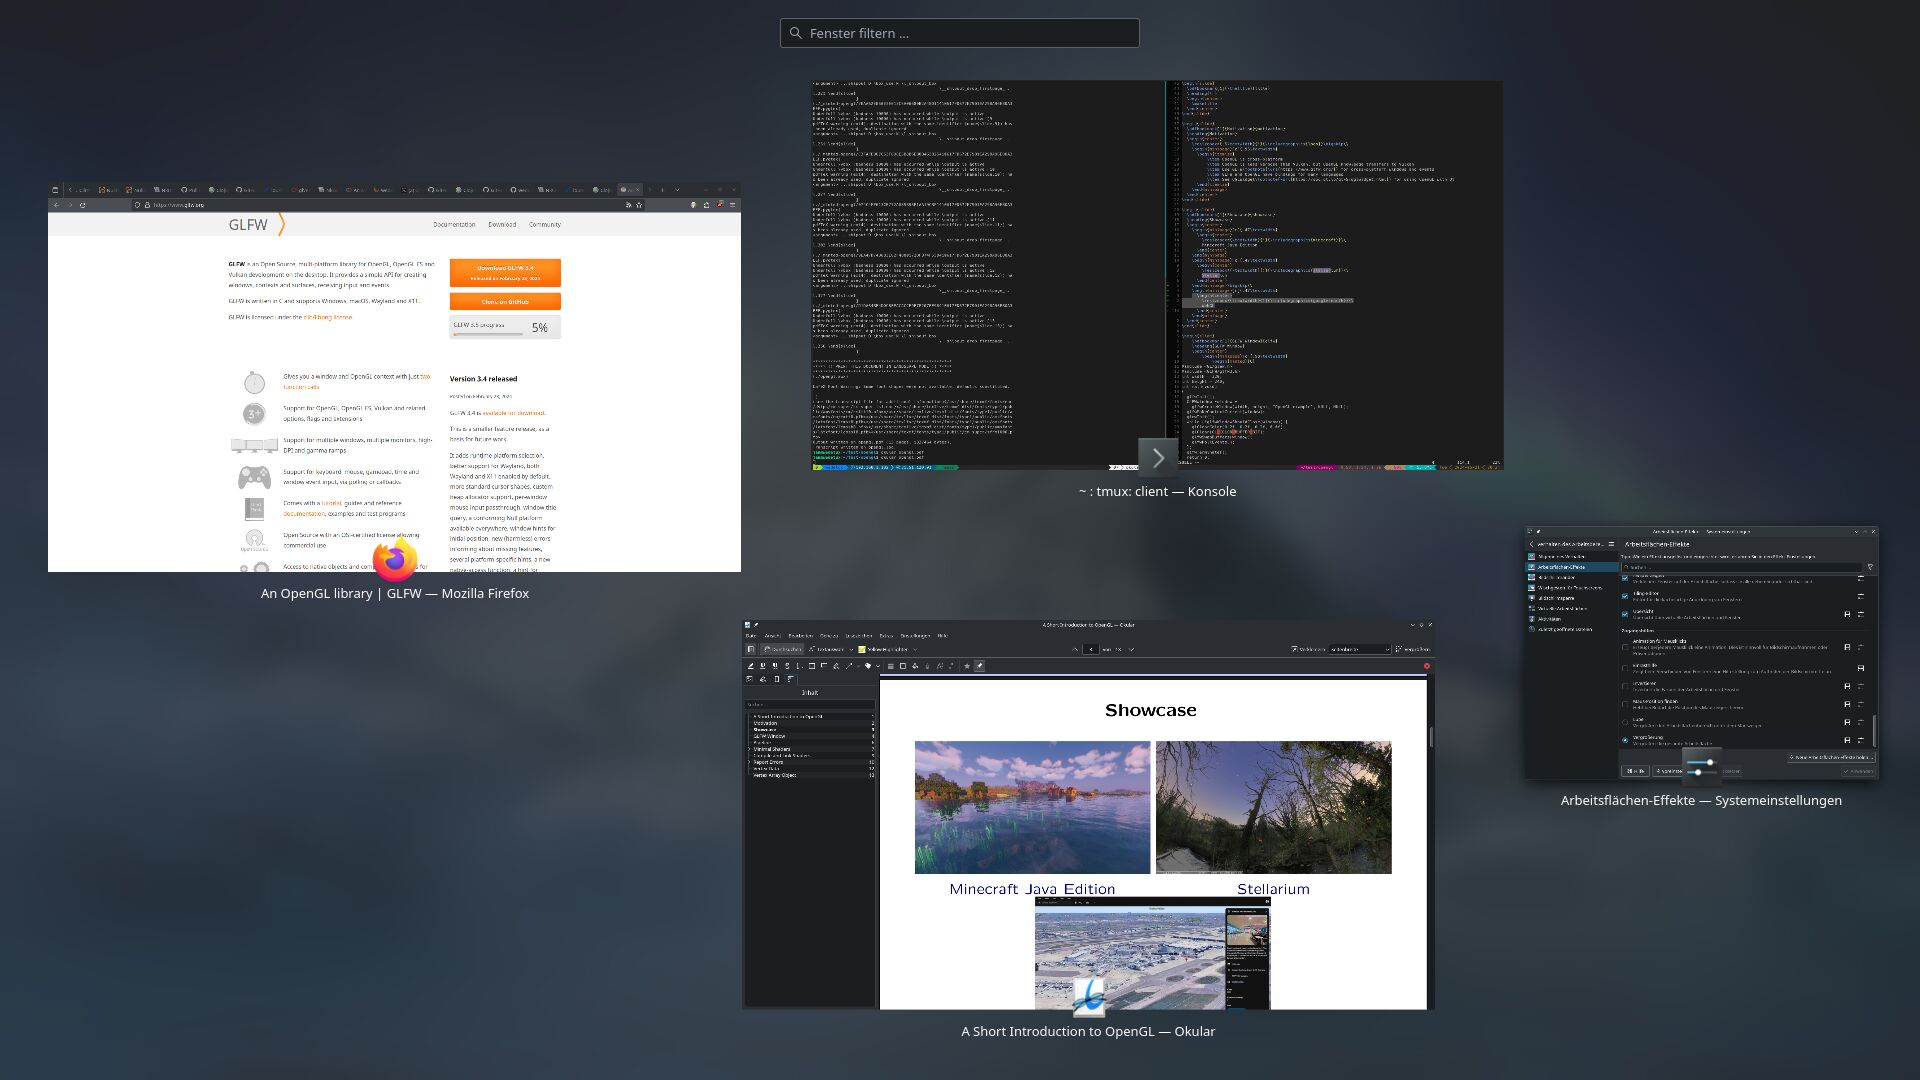
\includegraphics{kde}}\\
        KDE Plasma desktop
      \end{center}
    \end{minipage}
  \end{center}
\end{slide}

\begin{slide}
  \pdfbookmark[1]{GLEW}{glew}
  \heading{GLEW}
  \begin{center}
    \resizebox*{\textwidth}{!}{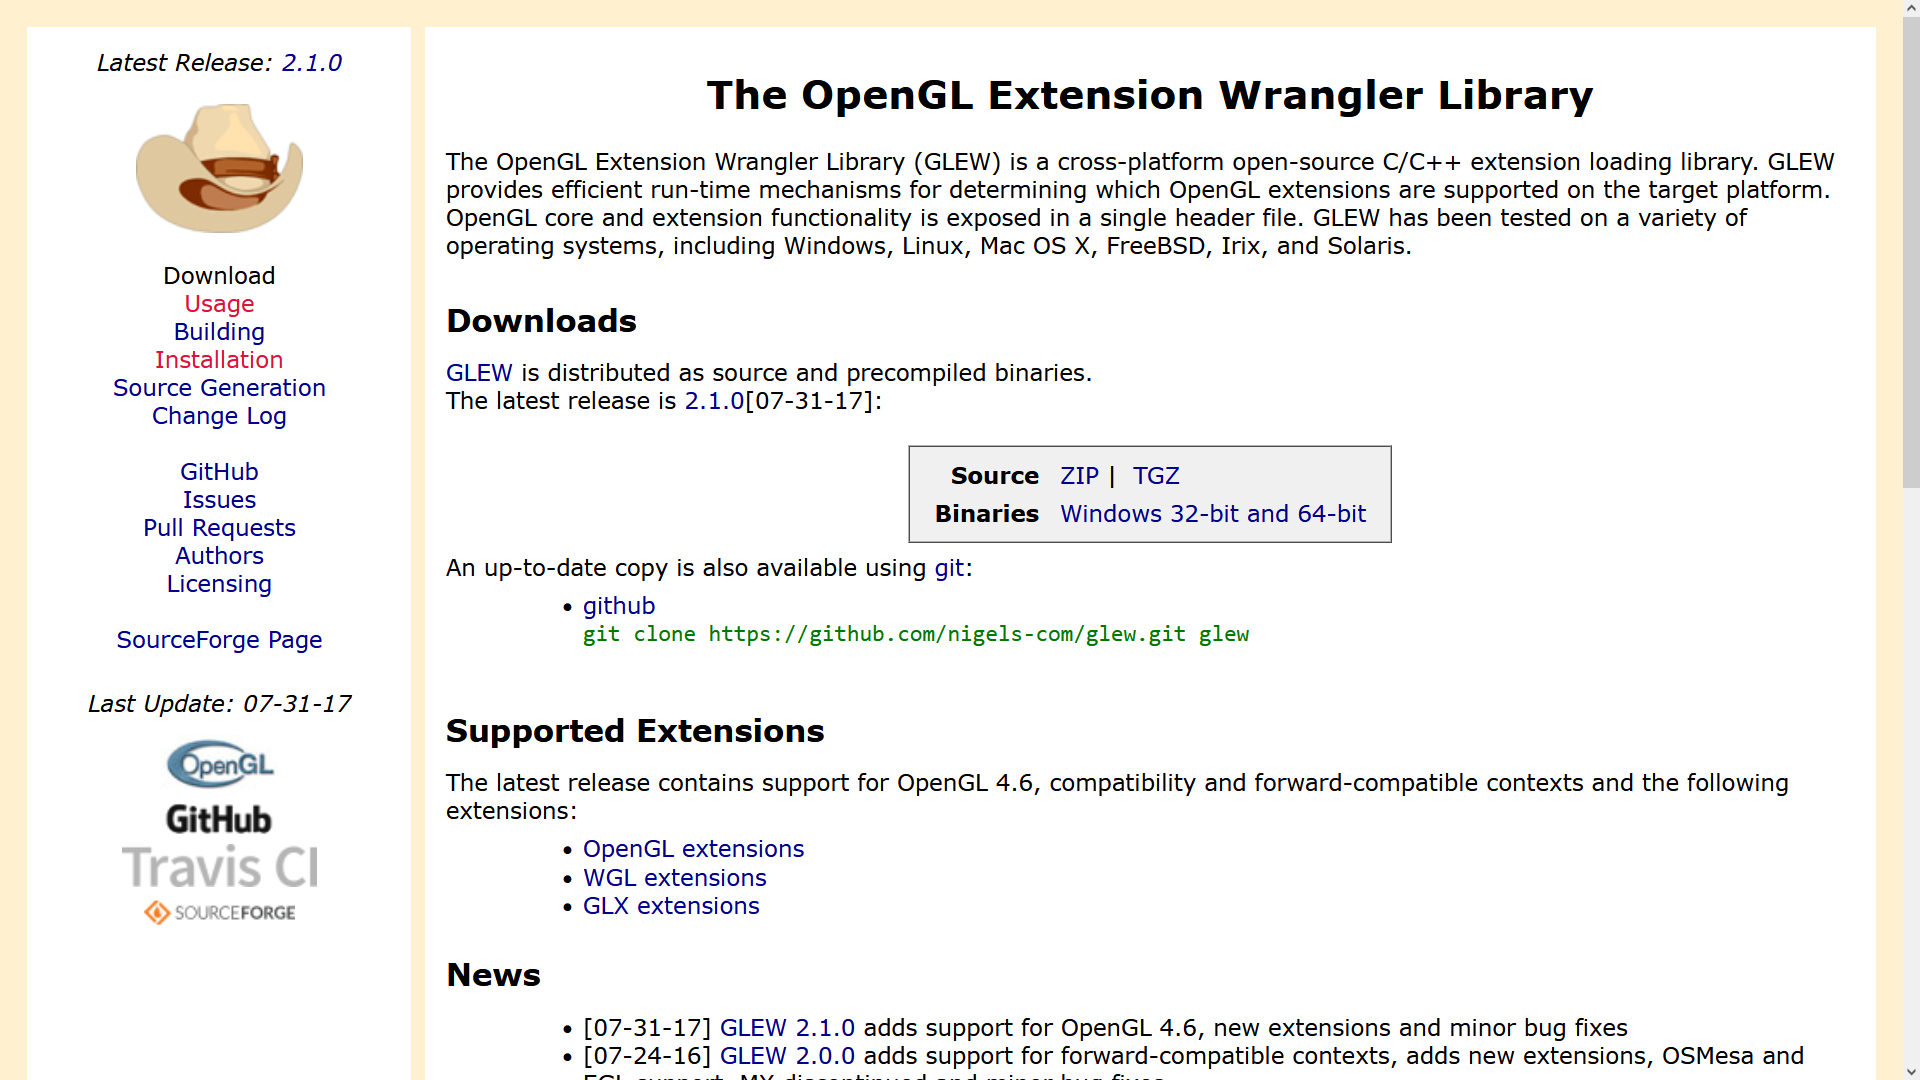
\includegraphics{glew}}\\
  \end{center}
\end{slide}

\begin{slide}
  \pdfbookmark[1]{GLFW}{glfw}
  \heading{GLFW}
  \begin{center}
    \resizebox*{\textwidth}{!}{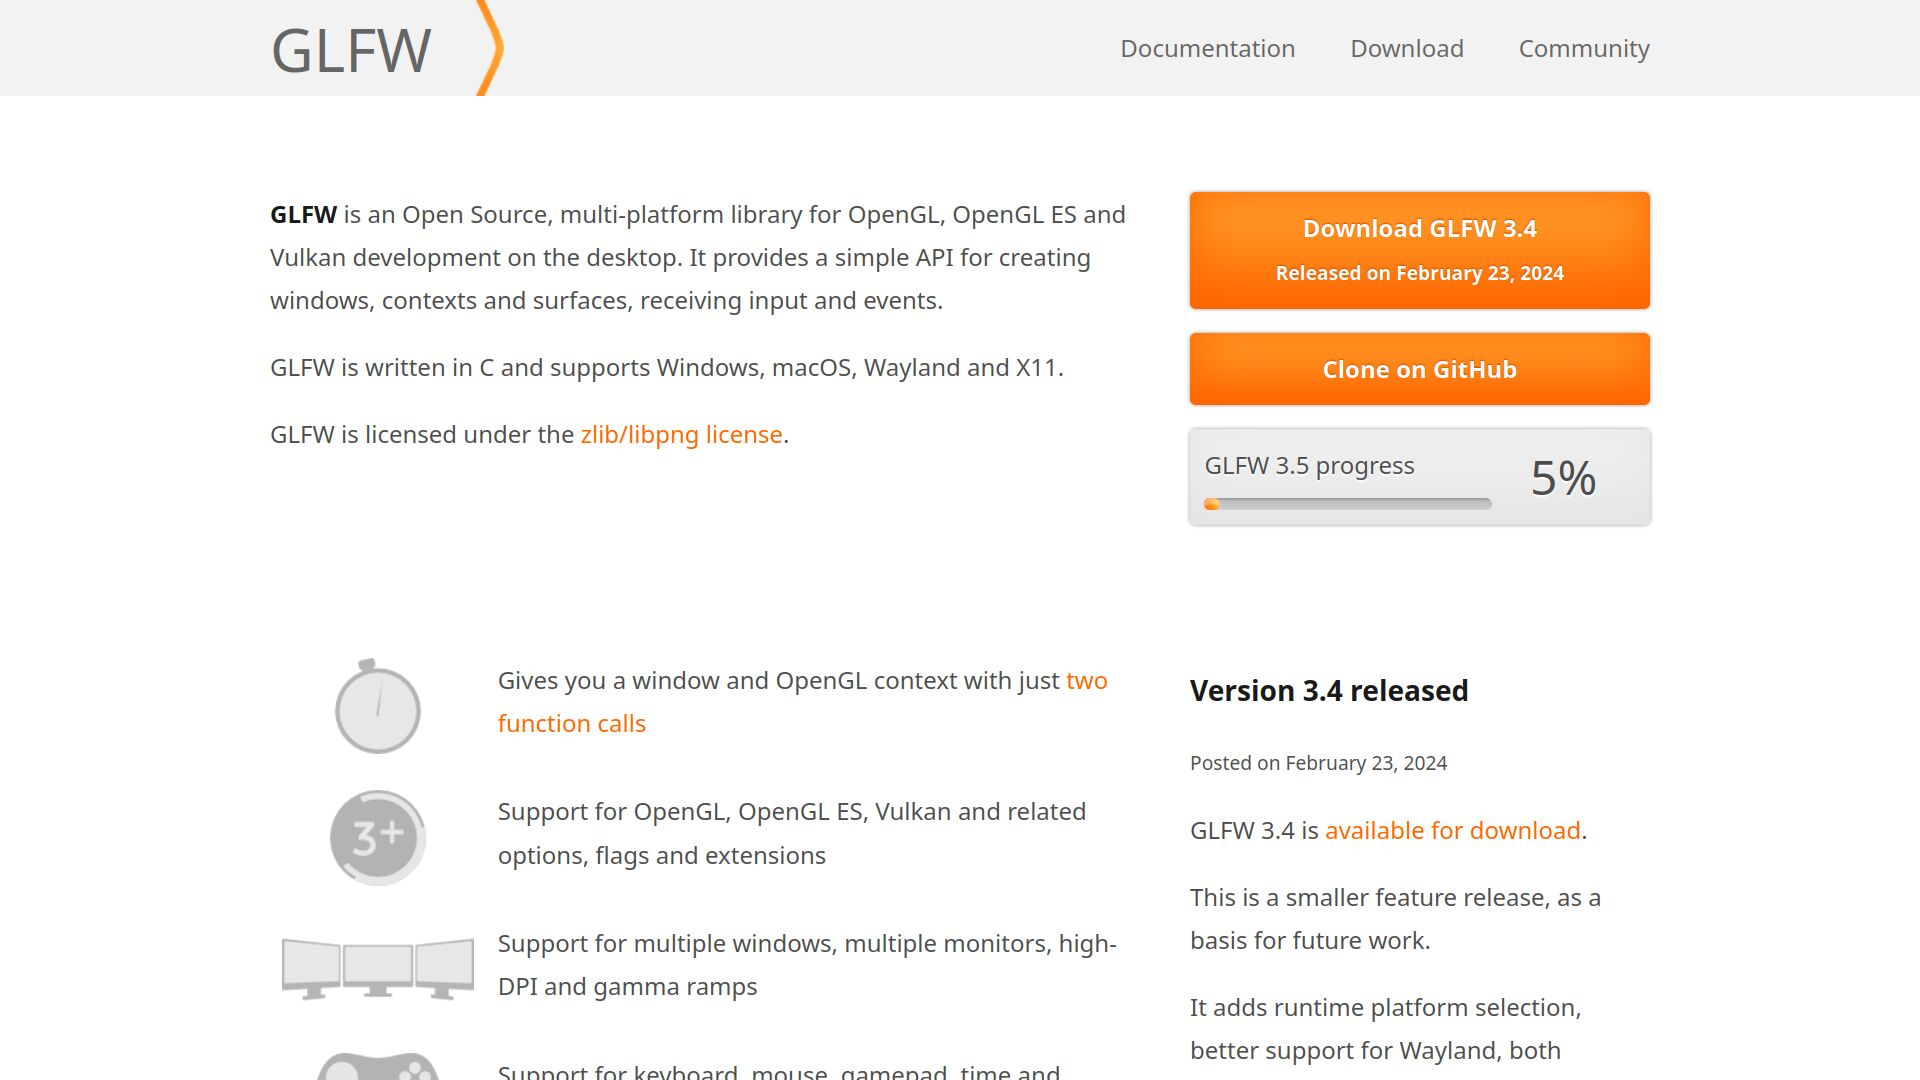
\includegraphics{glfw}}\\
  \end{center}
\end{slide}

\begin{slide}
    \pdfbookmark[1]{GLFW Window}{glfw}
    \heading{GLFW Window}
    \begin{center}
        \begin{minipage}[c]{.98\textwidth}
            \begin{minted}{C}
#include <GL/glew.h>
#include <GLFW/glfw3.h>
int width = 320;
int height = 240;
void main(void)
{
  glfwInit();
  GLFWwindow *window =
    glfwCreateWindow(width, height, "OpenGL example", NULL, NULL);
  glfwMakeContextCurrent(window);
  glewInit();
  glClearColor(0.2f, 0.2f, 0.2f, 0.0f);
  glViewport(0, 0, width, height);
  while (!glfwWindowShouldClose(window)) {
    glClear(GL_COLOR_BUFFER_BIT);
    glfwSwapBuffers(window);
    glfwPollEvents();
  };
  glfwTerminate();
}
            \end{minted}
        \end{minipage}
    \end{center}
\end{slide}

\begin{slide}
    \heading{GLFW Window}
    \begin{center}
      \resizebox*{.9\textwidth}{!}{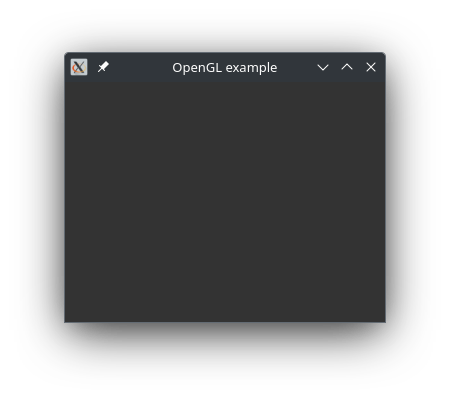
\includegraphics{glfw-window}}
    \end{center}
\end{slide}

\begin{slide}
  \pdfbookmark[1]{Minimal Pipeline}{minimal-pipeline}
  \heading{Minimal Pipeline}
  \begin{center}
    \resizebox*{.6\textwidth}{!}{
\includegraphics{pipeline-minimal}}
  \end{center}
\end{slide}

\begin{slide}
    \pdfbookmark[1]{Minimal Shaders}{shader}
    \pdfbookmark[2]{OpenGL Shader Language}{glsl}
    \heading{Minimal Shaders (OpenGL Shader Language (GLSL))}
    \begin{center}
        \begin{minipage}[c]{.5\textwidth}
            \begin{minted}{glsl}
#version 410 core
in vec3 point;
void main()
{
  gl_Position = vec4(point, 1);
}
            \end{minted}
            \vspace{-10pt}
            \rule{4cm}{0.4pt}
            \begin{minted}{glsl}
#version 410 core
out vec3 fragColor;
void main()
{
  fragColor = vec3(1, 0, 0);
}
            \end{minted}
        \end{minipage}
    \end{center}
\end{slide}

\begin{slide}
    \pdfbookmark[2]{Embedded in C}{shader}
    \heading{Minimal Shaders (Embedded in C)}
    \begin{center}
        \begin{minipage}[c]{.7\textwidth}
            \begin{minted}{C}
const char *vertexSource = "#version 410 core\n\
in vec3 point;\n\
void main()\n\
{\n\
  gl_Position = vec4(point, 1);\n\
}";

const char *fragmentSource = "#version 410 core\n\
out vec3 fragColor;\n\
void main()\n\
{\n\
  fragColor = vec3(1, 0, 0);\n\
}";
            \end{minted}
        \end{minipage}
    \end{center}
\end{slide}

\begin{slide}
    \pdfbookmark[1]{Compile and Link Shaders}{compile}
    \heading{Compile \& Link Shaders}
    \begin{center}
        \begin{minipage}[c]{.95\textwidth}
            \begin{minted}{C}
  // ...
  GLuint vertexShader = glCreateShader(GL_VERTEX_SHADER);
  glShaderSource(vertexShader, 1, &vertexSource, NULL);
  glCompileShader(vertexShader);
  handleCompileError("Vertex shader", vertexShader);

  GLuint fragmentShader = glCreateShader(GL_FRAGMENT_SHADER);
  glShaderSource(fragmentShader, 1, &fragmentSource, NULL);
  glCompileShader(fragmentShader);
  handleCompileError("Fragment shader", fragmentShader);

  GLuint program = glCreateProgram();
  glAttachShader(program, vertexShader);
  glAttachShader(program, fragmentShader);
  glLinkProgram(program);
  handleLinkError("Shader program", program);
  // ...
            \end{minted}
        \end{minipage}
    \end{center}
\end{slide}

\begin{slide}
    \pdfbookmark[1]{Report Errors}{report-errors}
    \pdfbookmark[2]{Compile Errors}{compile-error}
    \heading{Report Errors}
    \subheading{Compile Errors}
    \begin{center}
        \begin{minipage}[c]{.95\textwidth}
            \begin{minted}{C}
#include <stdio.h>
// ...
void handleCompileError(const char *step, GLuint context)
{
  GLint result = GL_FALSE;
  glGetShaderiv(context, GL_COMPILE_STATUS, &result);
  if (result == GL_FALSE) {
    char buffer[1024];
    glGetShaderInfoLog(context, 1024, NULL, buffer);
    if (buffer[0]) fprintf(stderr, "%s: %s\n", step, buffer);
  };
}
// ...
            \end{minted}
        \end{minipage}
    \end{center}
\end{slide}

\begin{slide}
    \pdfbookmark[2]{Link Errors}{link-error}
    \heading{Report Errors}
    \subheading{Link Errors}
    \begin{center}
        \begin{minipage}[c]{.95\textwidth}
            \begin{minted}{C}
#include <stdio.h>
// ...
void handleLinkError(const char *step, GLuint context)
{
  GLint result = GL_FALSE;
  glGetProgramiv(context, GL_LINK_STATUS, &result);
  if (result == GL_FALSE) {
    char buffer[1024];
    glGetProgramInfoLog(context, 1024, NULL, buffer);
    if (buffer[0]) fprintf(stderr, "%s: %s\n", step, buffer);
  };
}
// ...
            \end{minted}
        \end{minipage}
    \end{center}
\end{slide}

\begin{slide}
    \pdfbookmark[1]{Vertex Data}{vertex-data}
    \heading{Vertex and Index Data}
    \begin{center}
        \begin{minipage}[b]{.55\textwidth}
            \begin{minted}{C}
// ...
GLfloat vertices[] = {
  -0.5f, -0.5f,  0.0f,
   0.5f, -0.5f,  0.0f,
  -0.5f,  0.5f,  0.0f,
   0.5f,  0.5f,  0.0f
};

unsigned int indices[] = {0, 1, 3, 2};

GLuint vao;
GLuint vbo;
GLuint idx;
// ...
            \end{minted}
        \end{minipage}
        \begin{minipage}[b]{.4\textwidth}
          \resizebox*{.9\textwidth}{!}{
\includegraphics{ndc}}\\
          normalised device coordinates (NDC)
        \end{minipage}
    \end{center}
\end{slide}

\begin{slide}
    \pdfbookmark[1]{Vertex Array Object}{vao-data}
    \heading{Vertex Array Object}
    \begin{center}
        \begin{minipage}[c]{.95\textwidth}
            \begin{minted}{C}
  glGenVertexArrays(1, &vao);
  glBindVertexArray(vao);

  glGenBuffers(1, &vbo);
  glBindBuffer(GL_ARRAY_BUFFER, vbo);
  glBufferData(GL_ARRAY_BUFFER, sizeof(vertices), vertices,
               GL_STATIC_DRAW);
  glGenBuffers(1, &idx);
  glBindBuffer(GL_ELEMENT_ARRAY_BUFFER, idx);
  glBufferData(GL_ELEMENT_ARRAY_BUFFER, sizeof(indices), indices,
               GL_STATIC_DRAW);

  glVertexAttribPointer(glGetAttribLocation(program, "point"),
                        3, GL_FLOAT, GL_FALSE,
                        3 * sizeof(float), (void *)0);

  glUseProgram(program);
  glEnableVertexAttribArray(0);
            \end{minted}
        \end{minipage}
    \end{center}
\end{slide}

\begin{slide}
    \pdfbookmark[1]{Render Quads}{render-quads}
    \heading{Render Quads}
    \begin{center}
        \begin{minipage}[c]{.95\textwidth}
            \begin{minted}{C}
  // ...
  while (!glfwWindowShouldClose(window)) {
    glClear(GL_COLOR_BUFFER_BIT);
    glDrawElements(GL_QUADS, 4, GL_UNSIGNED_INT, (void *)0);
    glfwSwapBuffers(window);
    glfwPollEvents();
  };
  // ...
            \end{minted}
        \end{minipage}
    \end{center}
\end{slide}

\begin{slide}
    \heading{Render Quads}
    \begin{center}
      \resizebox*{.9\textwidth}{!}{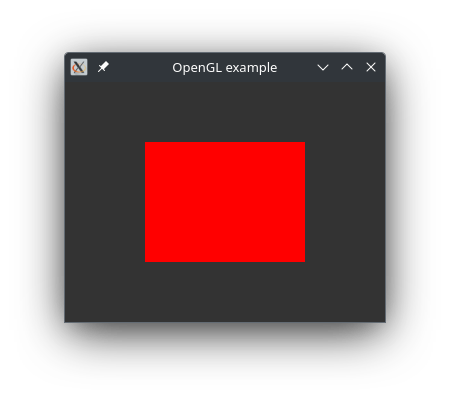
\includegraphics{quad}}
    \end{center}
\end{slide}

\begin{slide}
    \pdfbookmark[1]{Cleanup}{clean-up}
    \heading{Cleanup}
    \begin{center}
        \begin{minipage}[c]{.7\textwidth}
            \begin{minted}{C}
  // ...
  glDisableVertexAttribArray(0);

  glBindBuffer(GL_ELEMENT_ARRAY_BUFFER, 0);
  glDeleteBuffers(1, &idx);

  glBindBuffer(GL_ARRAY_BUFFER, 0);
  glDeleteBuffers(1, &vbo);

  glBindVertexArray(0);
  glDeleteVertexArrays(1, &vao);

  glDeleteProgram(program);
  glDeleteShader(vertexShader);
  glDeleteShader(fragmentShader);

  glfwTerminate();
  // ...
            \end{minted}
        \end{minipage}
    \end{center}
\end{slide}

\begin{slide}
    \pdfbookmark[1]{Texture Coordinates and Data}{texture-coords}
    \heading{Texture Coordinates and Data}
    \begin{center}
        \begin{minipage}[c]{.7\textwidth}
            \begin{minted}{C}
// ...
GLfloat vertices[] = {
  -0.5f, -0.5f,  0.0f, 0.0f, 0.0f,
   0.5f, -0.5f,  0.0f, 6.0f, 0.0f,
  -0.5f,  0.5f,  0.0f, 0.0f, 6.0f,
   0.5f,  0.5f,  0.0f, 6.0f, 6.0f
};

float chequer[] = {
  0.4f, 0.4f, 0.4f, 1.0f, 1.0f, 1.0f,
  1.0f, 1.0f, 1.0f, 0.4f, 0.4f, 0.4f
};
// ...
            \end{minted}
        \end{minipage}
    \end{center}
\end{slide}

\begin{slide}
    \pdfbookmark[2]{Shaders using Texture}{tex-shader}
    \heading{Shaders using Texture}
    \begin{center}
        \begin{minipage}[c]{.5\textwidth}
            \begin{minted}{glsl}
#version 410 core
in vec3 point;
in vec2 texcoord;
out vec2 UV;
void main()
{
  gl_Position = vec4(point, 1);
  UV = texcoord;
}
            \end{minted}
            \vspace{-10pt}
            \rule{4cm}{0.4pt}
            \begin{minted}{glsl}
#version 410 core
uniform sampler2D tex;
in vec2 UV;
out vec3 fragColor;
void main()
{
  fragColor = texture(tex, UV).rgb;
}
            \end{minted}
        \end{minipage}
    \end{center}
\end{slide}

\begin{slide}
    \pdfbookmark[1]{Multiple Vertex Attributes}{multiple-vertex}
    \heading{Multiple Vertex Attributes}
    \begin{center}
        \begin{minipage}[c]{.95\textwidth}
            \begin{minted}{C}
  // ...
  glVertexAttribPointer(glGetAttribLocation(program, "point"),
                        3, GL_FLOAT, GL_FALSE,
                        5 * sizeof(float),
                        (void *)0);
  glVertexAttribPointer(glGetAttribLocation(program, "texcoord"),
                        2, GL_FLOAT, GL_FALSE,
                        5 * sizeof(float),
                        (void *)(3 * sizeof(float)));
  glEnableVertexAttribArray(0);
  glEnableVertexAttribArray(1);
  // ...
            \end{minted}
        \end{minipage}
    \end{center}
\end{slide}

\begin{slide}
    \pdfbookmark[1]{2x2 Texture Setup}{texture-setup}
    \heading{2x2 Texture Setup}
    \begin{center}
        \begin{minipage}[c]{\textwidth}
            \begin{minted}{C}
  // ...
  GLuint tex;
  glGenTextures(1, &tex);
  glActiveTexture(GL_TEXTURE0);
  glBindTexture(GL_TEXTURE_2D, tex);
  glUniform1i(glGetUniformLocation(program, "tex"), 0);
  glTexImage2D(GL_TEXTURE_2D, 0, GL_RGB, 2, 2, 0, GL_BGR,
               GL_FLOAT, chequer);
  glTexParameteri(GL_TEXTURE_2D, GL_TEXTURE_WRAP_S, GL_REPEAT);
  glTexParameteri(GL_TEXTURE_2D, GL_TEXTURE_WRAP_T, GL_REPEAT);
  glTexParameteri(GL_TEXTURE_2D, GL_TEXTURE_MIN_FILTER, GL_NEAREST);
  glTexParameteri(GL_TEXTURE_2D, GL_TEXTURE_MAG_FILTER, GL_NEAREST);
  // ...
            \end{minted}
        \end{minipage}
    \end{center}
\end{slide}

\begin{slide}
    \pdfbookmark[1]{Texture Cleanup}{texture-cleanup}
    \heading{Texture Cleanup}
    \begin{center}
        \begin{minipage}[c]{.6\textwidth}
            \begin{minted}{C}
  // ...
  glBindTexture(GL_TEXTURE_2D, 0);
  glDeleteTextures(1, &tex);
  // ...
            \end{minted}
        \end{minipage}
    \end{center}
\end{slide}

\begin{slide}
    \pdfbookmark[1]{Textured Quad}{texture-quad}
    \heading{Textured Quad}
    \begin{center}
      \resizebox*{.9\textwidth}{!}{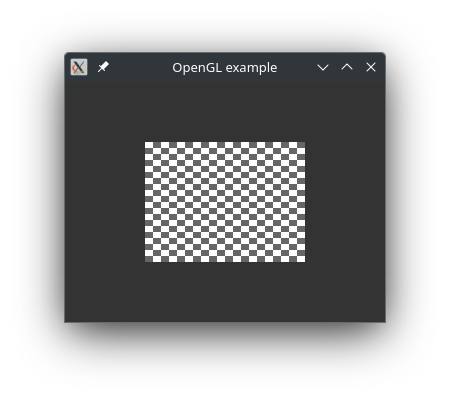
\includegraphics{chequer}}
    \end{center}
\end{slide}

\begin{slide}
    \pdfbookmark[1]{3D Rotations}{rotation}
    \heading{3D Rotations}
    \begin{center}
        \begin{minipage}[c]{.5\textwidth}
            \begin{minted}{glsl}
#version 410 core
uniform mat3 rotz;
uniform mat3 rotx;
in vec3 point;
in vec2 texcoord;
out vec2 UV;
void main()
{
  vec3 pos = rotx * rotz * point;
  gl_Position = vec4(point, 1);
  UV = texcoord;
}
            \end{minted}
        \end{minipage}
    \end{center}
\end{slide}

\begin{slide}
    \pdfbookmark[1]{Uniform Rotation Matrices}{uniform-rotation}
    \heading{Uniform Rotation Matrices}
    \begin{center}
        \begin{minipage}[c]{.95\textwidth}
            \begin{minted}{C}
#include <math.h>
// ...
  float alpha = 30 * M_PI / 180;
  float ca = cos(alpha);
  float sa = sin(alpha);
  float rotz[9] = {ca, sa, 0, -sa, ca, 0, 0, 0, 1};
  glUniformMatrix3fv(glGetUniformLocation(program, "rotz"),
                     1, GL_TRUE, rotz);

  float beta = 60 * M_PI / 180;
  float cb = cos(beta);
  float sb = sin(beta);
  float rotx[9] = {1, 0, 0, 0, cb, sb, 0, -sb, cb};
  glUniformMatrix3fv(glGetUniformLocation(program, "rotx"),
                     1, GL_TRUE, rotx);
  // ...
            \end{minted}
        \end{minipage}
    \end{center}
\end{slide}

\begin{slide}
    \pdfbookmark[1]{Rotated Quad}{rotated-quad}
    \heading{Rotated Quad}
    \begin{center}
      \resizebox*{.9\textwidth}{!}{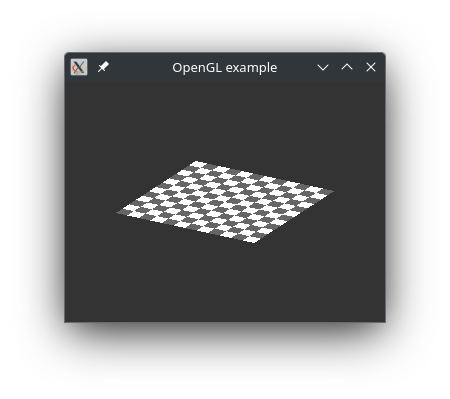
\includegraphics{rotated}}
    \end{center}
\end{slide}

\begin{slide}
    \pdfbookmark[1]{Enable Depth Testing}{depth-testing}
    \heading{Enable Depth Testing}
    \begin{center}
        \begin{minipage}[c]{.8\textwidth}
            \begin{minted}{C}
  glDepthFunc(GL_GEQUAL);
  glClipControl(GL_LOWER_LEFT, GL_ZERO_TO_ONE);
  glEnable(GL_DEPTH_TEST);
  glClearDepth(0.0);
  // ...
  while (!glfwWindowShouldClose(window)) {
    // ...
    glClear(GL_COLOR_BUFFER_BIT|GL_DEPTH_BUFFER_BIT);
    // ...
            \end{minted}
        \end{minipage}
    \end{center}
\end{slide}

\begin{slide}
    \pdfbookmark[1]{3D Projection Matrix}{projection}
    \heading{3D Projection Matrix}
    \begin{center}
        \begin{minipage}[c]{.45\textwidth}
            \resizebox*{\textwidth}{!}{
\includegraphics{frustum}}
        \end{minipage}
        {\Huge $\Rightarrow$}
        \begin{minipage}[c]{.45\textwidth}
            \resizebox*{\textwidth}{!}{
\includegraphics{ndcltd}}
        \end{minipage}\vspace{-16pt}\\
        $\mathcal{P}=
         \begin{pmatrix}
            dx & 0  &  0 & 0\\
            0  & dy &  0 & 0\\
            0  & 0  &  b & a\\
            0  & 0  & -1 & 0
        \end{pmatrix}$\medskip\\
        where
        $dx=\frac{1}{\tan(\frac{1}{2}fov)}$,
        $dy=\frac{width}{height}dx$,
        $a=\frac{far\cdot near}{far-near}$,
        $b=\frac{near}{far-near}$\bigskip\\
        \url{https://www.wedesoft.de/software/2021/09/20/reversed-z-rendering/}
    \end{center}
\end{slide}

\begin{slide}
    \pdfbookmark[1]{Shader with Translation and Projection}{shader-projection}
    \heading{Shader with Translation and Projection}
    \begin{center}
        \begin{minipage}[c]{.65\textwidth}
            \begin{minted}{glsl}
#version 410 core
uniform mat3 rotz;
uniform mat3 rotx;
uniform mat4 projection;
uniform float distance;
in vec3 point;
in vec2 texcoord;
out vec2 UV;
void main()
{
  vec3 pos = rotx * rotz * point;
  pos.z -= distance;
  gl_Position = projection * vec4(pos, 1);
  UV = texcoord;
}
            \end{minted}
        \end{minipage}
    \end{center}
\end{slide}

\begin{slide}
    \pdfbookmark[1]{Uniform Distance and Projection Matrix}{uniform-projection}
    \heading{Uniform Distance and Projection Matrix}
    \begin{center}
        \begin{minipage}[c]{.95\textwidth}
            \begin{minted}{C}
  // ...
  glUniform1f(glGetUniformLocation(program, "distance"), 1.8);

  float fov = 45.0 * M_PI / 180;
  float near = 0.1;
  float far = 10.0;
  float dx = 1.0 / tan(0.5 * fov);
  float dy = dx * width / height;
  float a = far * near / (far - near);
  float b = near / (far - near);
  float projection[16] = {dx, 0, 0, 0, 0, dy, 0, 0,
                          0, 0, b, a, 0, 0, -1, 0};
  glUniformMatrix4fv(glGetUniformLocation(program, "projection"),
                     1, GL_TRUE, projection);
  // ...
            \end{minted}
        \end{minipage}
    \end{center}
\end{slide}

\begin{slide}
    \pdfbookmark[1]{Projected Quad}{projected-quad}
    \heading{Projected Quad}
    \begin{center}
      \resizebox*{.9\textwidth}{!}{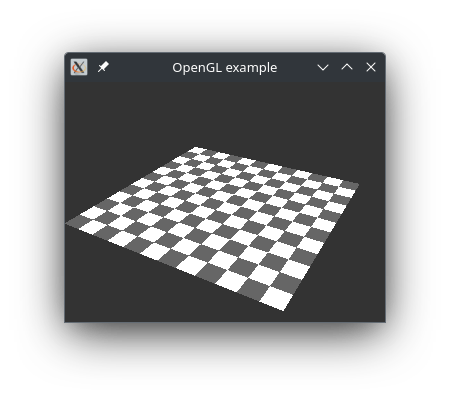
\includegraphics{projected}}
    \end{center}
\end{slide}

\begin{slide}
  \pdfbookmark[1]{Full Pipeline}{full-pipeline}
  \heading{Full Pipeline}
  \begin{center}
    \resizebox*{.6\textwidth}{!}{
\includegraphics{pipeline}}
  \end{center}
\end{slide}

\begin{slide}
    \pdfbookmark[1]{Tessellation}{tessellation}
    \heading{Tessellation}
    \begin{center}
        \begin{minipage}[c]{.45\textwidth}
            \resizebox*{\textwidth}{!}{
\includegraphics{original}}
        \end{minipage}
        {\Huge $\Rightarrow$}
        \begin{minipage}[c]{.45\textwidth}
            \resizebox*{\textwidth}{!}{
\includegraphics{tessellation}}
        \end{minipage}
    \end{center}
\end{slide}

% Tessellation (radial sinc wave)
% Phong shading of quad
% clean up texture

\begin{slide}
  \pdfbookmark[1]{Further Topics}{further}
  \heading{Further Topics}
  \begin{center}
    \begin{minipage}[c]{.6\textwidth}
      \begin{itemize}
        \item Face culling
        \item Fog
        \item Shadow mapping
        \item Volumetric rendering
        \item glTF asset import (e.g. using Assimp)
      \end{itemize}
    \end{minipage}
  \end{center}
\end{slide}

\begin{slide}
  \pdfbookmark[1]{OpenGL Superbible}{superbible}
  \heading{OpenGL Superbible}
  \begin{center}
    \resizebox*{.45\textwidth}{!}{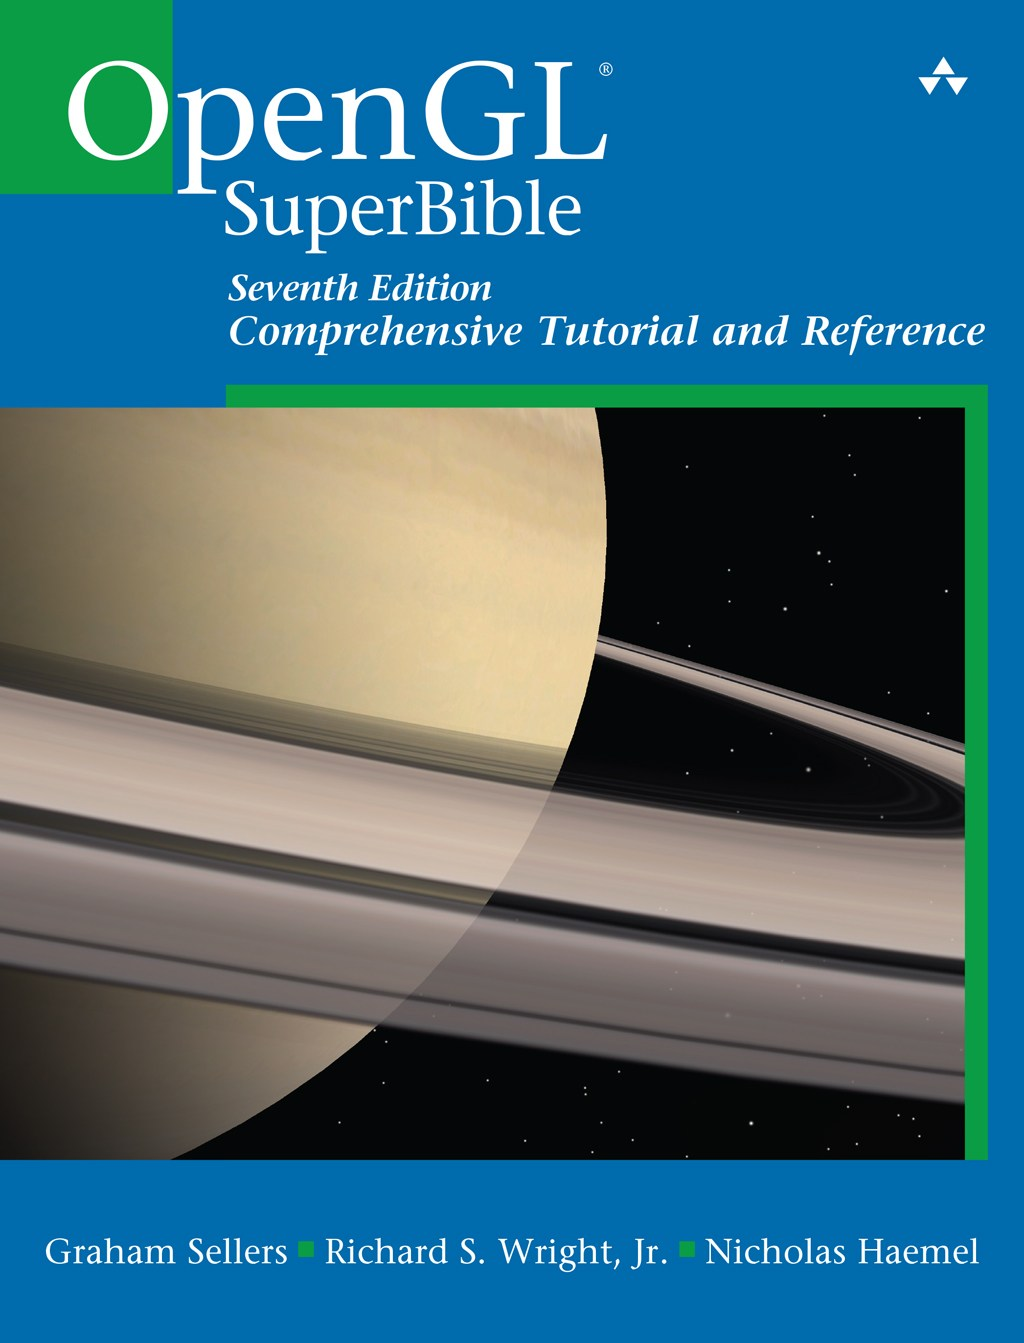
\includegraphics{superbible}}\\
    {\small \url{https://www.informit.com/store/opengl-superbible-comprehensive-tutorial-and-reference-9780134193137}}
  \end{center}
\end{slide}

\begin{slide}
  \pdfbookmark[1]{Learn OpenGL}{learnopengl}
  \heading{Learn OpenGL}
  \begin{center}
    \resizebox*{.45\textwidth}{!}{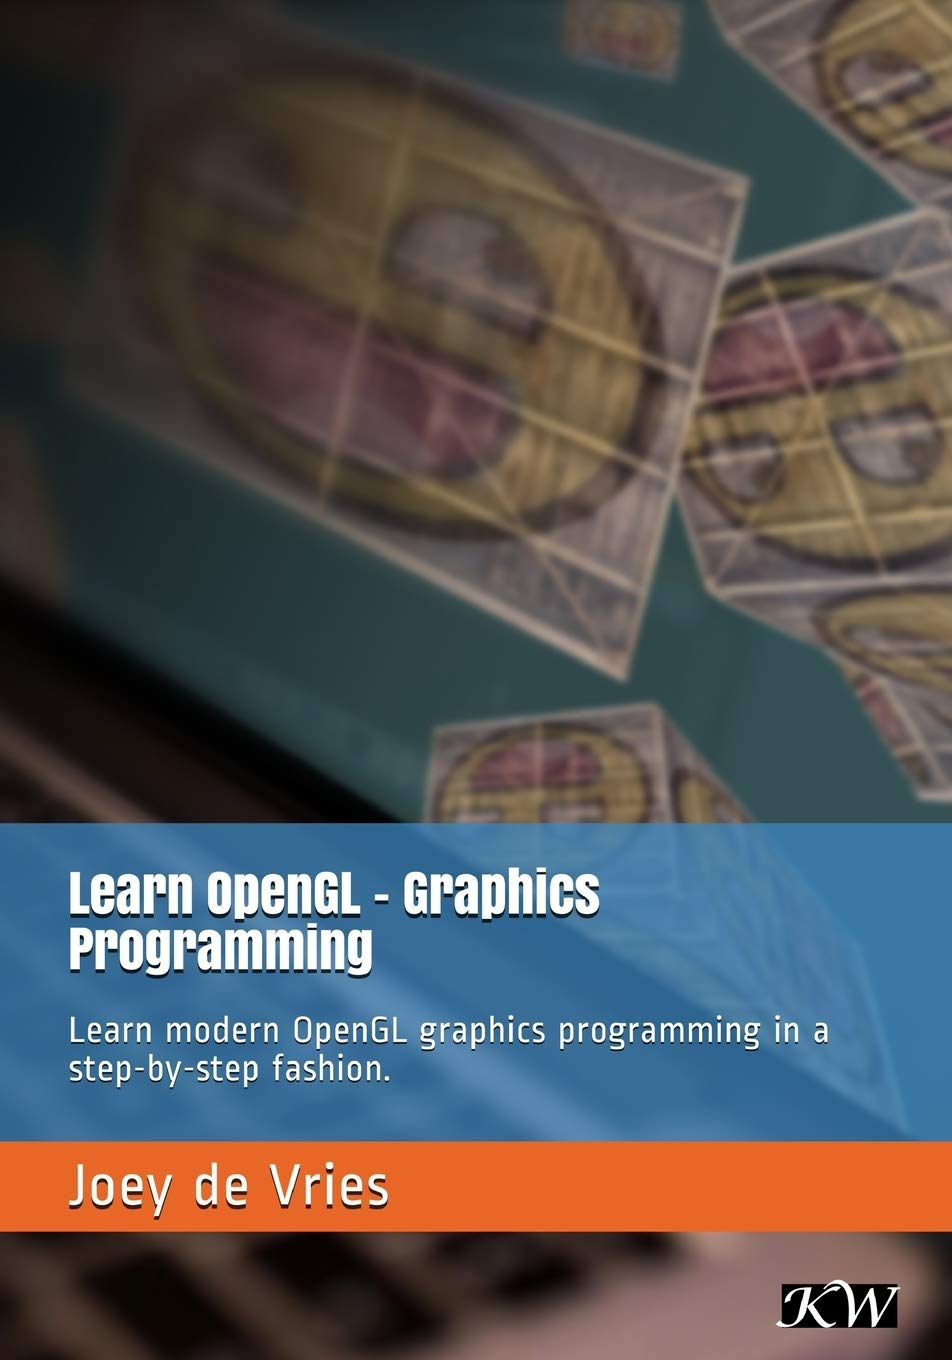
\includegraphics{learnopengl}}\\
    \url{https://learnopengl.com/}
  \end{center}
\end{slide}

\end{document}
